\documentclass{standalone}

\usepackage{tikz}
\usepackage{circuitikz}

\tikzset{block/.style = {draw, fill=white, very thick, rectangle, minimum height=1cm, minimum width=2cm},
         lblock/.style={draw,fill=white,very thick, rectangle, minimum height=3cm, minimum width=1cm},
         sum/.style= {draw, fill=white, very thick, circle, node distance=0.5cm}}

         
\begin{document}
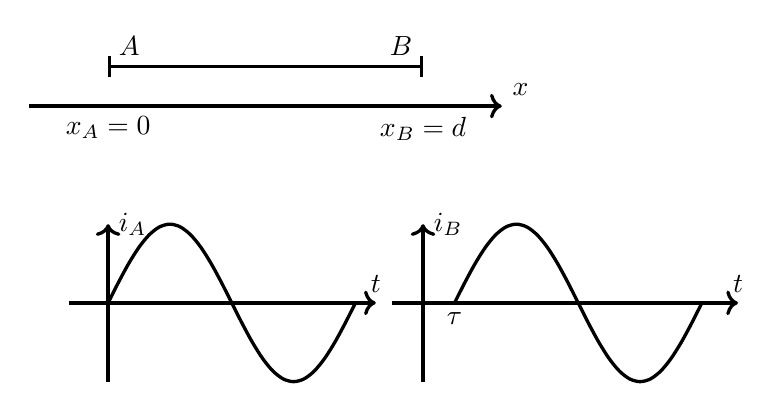
\begin{tikzpicture}[scale=2]
    \draw[|-|,very thick](0,0)node[above right]{$A$}--(2,0)node[above left]{$B$};
    \draw[->,very thick](-0.5,-0.25)--(0,-0.25)node[below]{$x_A=0$}--(2,-0.25)node[below]{$x_B=d$}--(2.5,-0.25)node[above right]{$x$};

    \draw[->,very thick](0,-2)--(0,-1)node[right]{$i_A$};
    \draw[->,very thick](-0.25,-1.5)--(1.7,-1.5)node[above]{$t$};
    \draw[-,very thick]plot[smooth, domain=0:1.57](\x,{1/2*sin(4*\x r)-1.5});

    \draw[->,very thick](2,-2)--(2,-1)node[right]{$i_B$};
    \draw[->,very thick](1.8,-1.5)--(4,-1.5)node[above]{$t$};
    \draw[-,very thick]plot[smooth, domain=2.2:3.77](\x,{1/2*sin(4*(\x-2.2) r)-1.5});
    \node[below]at(2.2,-1.5){$\tau$};
\end{tikzpicture}
\end{document}